%\setcounter{section}{2}
\section{国際SKAのサイエンス}\label{c03.s2}
\input{EoR/c03/c03.s2.ss1.tex}%再電離の物理
\input{EoR/c03/c03.s2.ss2.tex}%再電離期のモデリングとSKAへ向けたシミュレーション
\subsection{$B=iBe6d2O!"(BLyman-$\alpha$$B$H(BX$B@~6/EY$NMI$i$.!"%9%T%s29EY(B}
\label{c03.s2.ss3}
\begin{figure}[!t]
	\centering
	{\includegraphics[width=8cm]{EoR/c03/c03.s2.f3.eps}}
	\caption{$B%7%_%e%l!<%7%g%s$K$h$C$FF@$i$l$?=iBe@1=i4|<ANL4X?t$N0l(B
 $BNc(B \citep{2014ApJ...792...32S}$B!#$3$N7W;;$G$O!"E57?E*$K$O(B$10-100M_\odot$$B!"3d9g$O>/$J$$$,(B$>100M_\odot$$B$d(B$<10M_\odot$$B$N=iBe@1$bB8:_!#$*$h$=(B1/3$B$,C1FH@1!"$=$l0J30$G$OJ#?t$N@17O$H$7$FCB@8!#(B}\label{KH3}
\end{figure}

\begin{figure}[!h]
	\centering\vspace*{1cm}
	{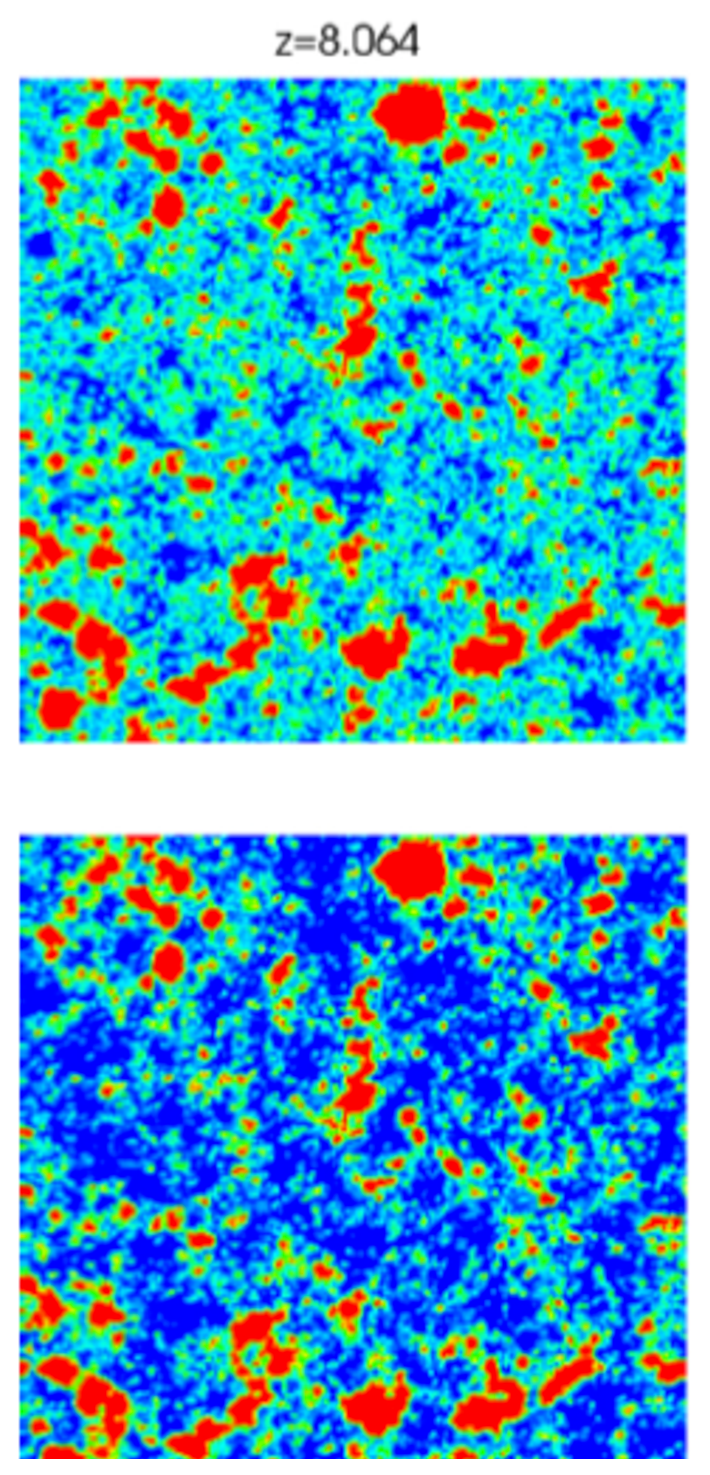
\includegraphics[width=5cm,angle=90]{EoR/c03/c03.s2.f4.eps}}
	\caption{$B%_%K%O%m!<$r9MN8$7$?>l9g(B($B:8?^(B)$B$H9MN8$7$J$$>l9g(B($B1&?^(B)$B$N(B
 $B@VJ}JP0\(B$z\approx8$$B$G$NEEN%9=B$(B($B@V$,EEN%NN0h!"@D$,Cf@-NN0h(B)$B!#%_%K%O%m!<(B
 $B$r9MN8$7$?>l9g!"ItJ,EEN%$5$l$?NN0h(B($BNP$NNN0h(B)$B$,@j$a$kBN@Q$,B?$/$J$j!"%H(B
 $B%`%=%s;6Mp$N8w3XE*8|$,A}2C$9$k(B \citep{2012ApJ...756L..16A}$B!#(B}\label{KH2} 
\end{figure}

EoR$B$N=i4|CJ3,$d(BCD$B$O!"=iBe@17A@.$K$h$C$F;O$^$k!#=iBe@1$O!"%_%K%O%m!<(B
($T_{\rm vir}<10^4$K, $B$b$7$/$O(B $10^4<M/M_\odot < 10^{7-8}$)$BFb$G@8$^$l$k$H?.$8$i(B
$B$l$F$$$k$,!"$3$N:]!"=iBe@1$N7A@.$O<g$K?eAGJ,;RNd5Q$K$h$C$F0z$-5/$3$5$l!"(B
$B8=:_$N@1(B($B<oB2(BI$B@1(B)$B$H$O0[$J$j=E85AG$r4^$^$J$$;v$+$i<oB2(BIII$B@1(B(Population
III star)$B$H$b8F$P$l$k(B\footnote{$B=E85AG$r4^$^$J$$@1$G$"$C$F$b!"@17A@.NN0h$,(B
$BEEN%!&2rN%mU<M$N1F6A$r<u$1$F$$$J$$>l9g$K$O<oB2(BIII.1$B@1!"$3$l$i$N1F6A$r<u$1(B
$B$?8e$K7A@.$5$l$k<!@$Be$N@1$O<oB2(BIII.2$B@1$H6hJL$9$k(B
\citep{2008AIPC..990.....O}$B!#$=$N0UL#$G!"<oB2(BIII$B@1$H=iBe@1$NDj5A$O87L)$K(B
$B$O0lCW$7$J$$!#(B}$B!#(B

\begin{figure}[!t]
	\centering
	{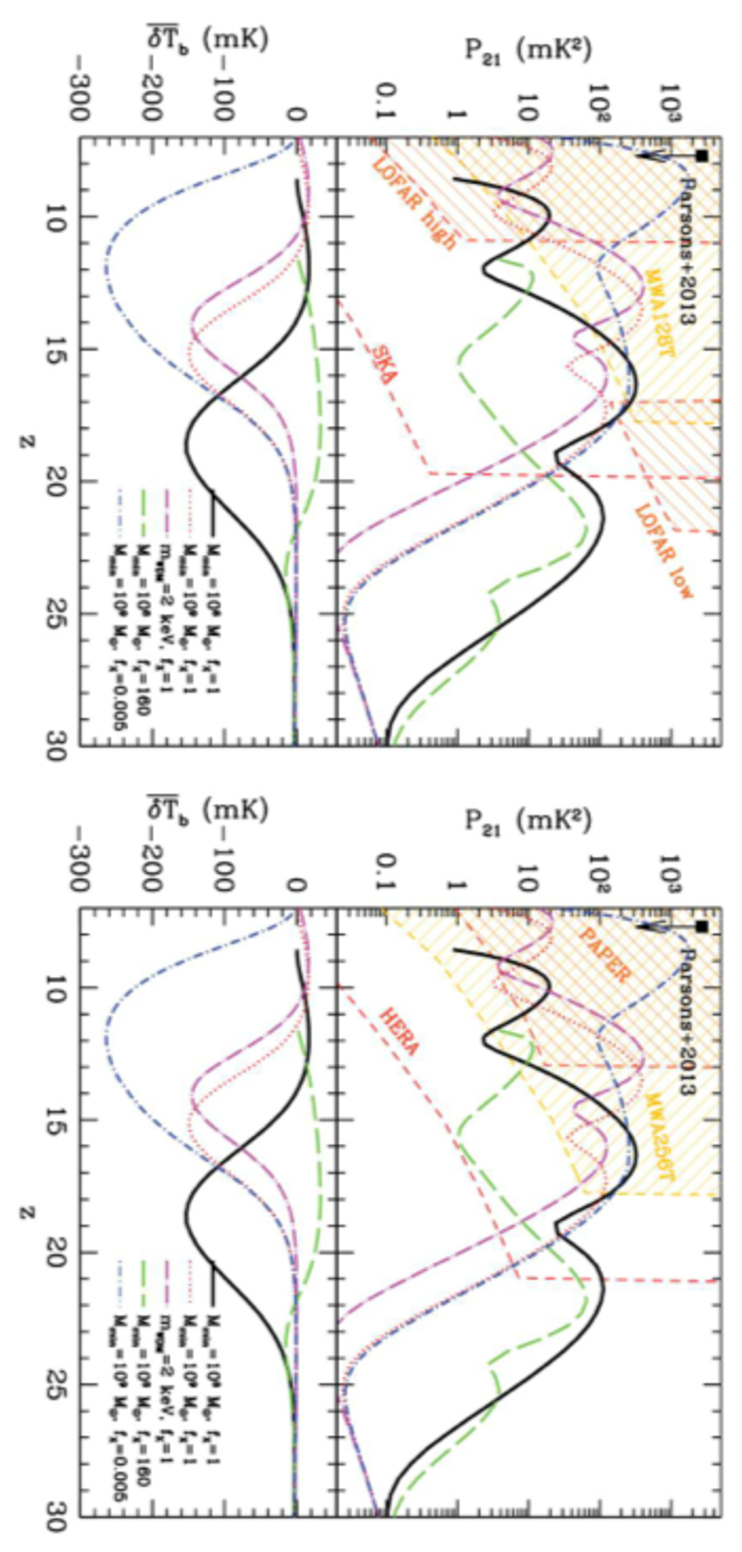
\includegraphics[width=5cm, angle=90]{EoR/c03/c03.s2.f5.eps}}
	\caption{$B>eCJ(B: $k=1/\rm Mpc$$B$K$*$1$k5eJ?6Q$7$?%Q%o!<%9%Z%/%H%k(B$P_{21}$$B$N?J2=(B $B!#$3$3$G!"(B$P_{21}$$B$O!"(B$P_{21}\equiv k^3/(2\pi^2V) \overline{\delta T_b}(z)^2\langle |\delta_{21}({\bf k},z)|^2 \rangle_k $$B!"(B$\delta_{21}({\bf x},z)=\delta T_b({\bf x},z)/\overline{\delta T_b}(z)-1$$B$GDj5A$5$l$k!#2<CJ(B: $BJ?6Q(B$\delta T_b$$B$N?J2=(B}\label{KH4}
\end{figure}
\begin{figure}[!h]
	\centering
	{\includegraphics[width=5cm, angle=270]{EoR/c03/c03.s2.f6.eps}}
	\caption{$B:8?^(B: $BM}A[$J>u67$G$N<oB2(BIII$B@1(B + X$B@~8;$r4^$`6d2O<~$j$N%,(B
 $B%929EY(B($BGK@~(B)$B$H%9%T%s29EY(B($B<B@~(B)($B2<CJ(B)$B$H(B$\delta T_b$($B>eCJ(B) \citep{2008ApJ...684...18C}$B!#1&?^(B: $B$"$k$R$H$D$N1'ChO@E*L)EY%T!<%/(B $B$G7A@.$5$l$?L)=8$7$?6d2OFb$K<oB2(BIII$B@1(B + X$B@~O"@1(B + $B<oB2(BII$B@1$,B8:_$7$?>l9g$N(B$\delta T_b$$BJ,I[(B \citep{2014arXiv1405.2085A}$B!#(B $B%7%_%e%l!<%7%g%sNN0h%5%$%:$O!"0lJU(B40 comoving Mpc$B$G(B, $B%S!<%`I}(B $\Theta=2'$$BAjEv$NJ?3j2=$r9T$C$?8e$N?^$G$"$k!#?^Cf?4$NL)EY%T!<%/%5%$%:$O(B$\sim7$Mpc$\sim 10'$$B$KAjEv$9$k!#:8?^$G$O!"EEN%NN0h$9$030(B($BEEN%GHLL(B)$B$G2CG.$K$h$k51@~NN0h(B, $B$=$N$^$o$jNd$?$$%,%9$K$h$k5[<}NN0h$,8+$($k!#1&?^$G$O(B$\delta T_b>0$$B$N51@~NN0h$,8+$($J$$$,!"%S!<%`I}$r>.$5$/$7$?>l9g(B($B6u4VJ,2rG=$r>e$2$?>l9g(B)$B$K$O8+$($k2DG=@-$b$"$k!#(B}
	\label{KH5}
\end{figure}

2000$BG/:"$h$j?tCM%7%_%e%l!<%7%g%s$K$h$k=iBe@17A@.$N8&5f$,3hH/$K$J$j!"Bg<A(B
$BNL(B($\ge100M_\odot$)$B$N<oB2(BIII$B@1$,8IN)$7$F7A@.$5$l$k!"$$$o$f$k!H(Bone Pop III
star per one minihalo$B!I%Q%i%@%$%`$,?.$8$i$l$F$-$?(B(e.g.,
\cite{2002Sci...295...93A, 2002ApJ...564...23B, 2006ApJ...652....6Y}) $B!#(B
$B6aG/$G$O!"B??t$N%_%K%O%m!<%5%s%W%k$rMQ$$$?%7%_%e%l!<%7%g%s$K$h$C$FI}9-$$(B
$B<oB2(BIII$B@1<ANL$,<B8=$5$l$k;v$b<($5$l(B(e.g., \cite{2014ApJ...781...60H},
\cite{2014ApJ...792...32S})$B!"0l$D$N%_%K%O%m!<Fb$GJ#?t$NHf3SE*7Z$$(B
($10-100M_\odot$)$B@1$,@8$^$l$k2DG=@-$b;XE&$5$l$F$$$k(B(e.g.,
\cite{2009Sci...325..601T, 2010MNRAS.403...45S, 2011ApJ...737...75G,
2014ApJ...792...32S}, $B?^(B\ref{KH3})\footnote{$B6aG/$N798~$H$7$F$O%_%K%O%m!<(B
$BFb$N%,%9J,Nv$O5/$3$j$&$k$H$$$&8+J}$,B?$$!#$7$+$7!"$=$l$iJ,NvJR$,@1$K$J$k(B
$B$+!"$b$7$/$O$=$N$^$^Cf?4@1$K9_Ce$9$k$+$O$^$@5DO@$,<}B+$7$F$$$J$$!#(B}$B!#<oB2(B
III$B@1$N=i4|<ANL4X?t(B(Initial Mass Function: IMF) $B$O!"$3$l$i@1$+$i$NJ|<M$N(B
$B%9%Z%/%H%k%(%M%k%.!<J,I[(B(Spectral Energy Distribution: SED)$B$N9E$5(B
(hardness)$B$K4XO"$9$k!#$^$?!"(BX$B@~O"@1$,7A@.$5$l$k>l9g!"(BX$B@~$NBg$-$JJ?6Q<+M3(B
$B9TDx$K$h$j!";g30@~$GEEN%$5$l$k>l9g$HHf$Y$F$J$a$i$+$JEEN%9=B$$,$G$-$k$H9M(B
$B$($i$l$k(B \citep{2013MNRAS.431..621M}$B!#$3$N$h$&$K!"<oB2(BIII$B@1$N(BIMF$B$d7A@.N($O(B
$BEEN%9=B$$NH/C#$HL)@\$K4XO"$9$k!#(B



$B$7$?$,$C$F!"=iBe@17A@.!&?J2=$NM}O@$O(BCD, EoR$B$N%b%G%j%s%0$N:]$K=EMW$H$J$k!#(B
$B=iBe@17A@.$K$*$$$F!"<g$K$=$N7A@.$rAK32$9$k$N$O(BLyman-Werner$B%P%s%ImU<M$K$h(B
$B$k?eAGJ,;R$N8w2rN%$G$"$j(B(e.g., \cite{2000ApJ...534...11H})$B!"6aG/$G$O!"$3(B
$B$N?eAGJ,;R2rN%8w;R$NmU<MM"Aw$b9MN8$7$?BgNN0h(B($\ge 100$Mpc)$B:FEEN%%7%_%e%l!<(B
$B%7%g%s$b$J$5$l$F$$$k(B (\cite{2012ApJ...756L..16A} $B?^(B\ref{KH2})$B!#(B 



$B$^$?6aG/$G$O!"@2$l>e$,$j4|$K$*$1$k%P%j%*%s$H%@!<%/%^%?!<$NB.EY:9$N8z2L$b(B
$BE7BN7A@.2aDx$K1F6A$rM?$($k$H9M$($i$l$F$$$k(B \citep{2010PhRvD..82h3520T}$B!#(B
$B$3$N8z2L$r9MN8$7$?>l9g!"@17A@.2DG=$J%_%K%O%m!<<ANL$,Bg$-$/$J$j!"%O%m!<$N(B
$B7A@.;~4|$bCY$/$J$k;v$,?tCM%7%_%e%l!<%7%g%s$K$h$C$F<($5$l$F$$$k(B
 \citep{2011ApJ...730L...1S, 2011ApJ...736..147G}$B!#$^$?!"$3$NB.EY:9$N8z2L(B
$B$O!">W7bGH$h$C$FBg6IE*$J2CG.$r0z$-5/$3$9;v$G(B21 cm $B%Q%o!<%9%Z%/%H%k$K1F6A(B
$B$rM?$($k;v$b9M$($i$l$k(B \citep{2012ApJ...760....3M}$B!#(B

CD$B$H(BEoR$B$K$*$1$k(B21 cm$B%Q%o!<%9%Z%/%H%k2r@O$K4X$7$F!";0$D$NFCD'E*$J;~4|$,$"(B
$B$k!#(B(1) IGM$B$N29EY$,!"(BWouthysen-Field$B8z2L$K$h$C$F(BLyman-$\alpha$$BmU<M$H6/$/(B
$B%+%C%W%k$9$k!V(BLyman-$\alpha$-pumping epoch$B!W(B, (2) IGM$B$,(BX$B@~$K$h$C$F2CG.$5(B
$B$l!"=y!9$K(BCMB$B29EY$rD6$($k!V(BX-ray heating epoch$B!W!"(B(3) $BEEN%%P%V%k$,1'ChO@(B
$BE*%9%1!<%k$G7A@.$5$l$k!V(BEpoch of Reionization$B!W!#$=$l$>$l$N;~4|$G!"(B21 cm
$B51EY29EY(B ($\delta T_b\equiv{(T_{\rm
s}-T_{\gamma}(z))}(1-e^{-\tau_{21}})/(1+z))$)$B$N?6I}$d6u4VMI$i$.$OA}I}$5$l(B
$B$k(B (\cite{2014MNRAS.439.3262M}, $B?^(B\ref{KH4})$B!#(B 

$B:$Fq$G$O$"$k$,!"%H%b%0%i%U%#!<(B($B3F@VJ}JP0\$G$N;#A|(B)$B$O=iBe6d2O$[$I>.$5$JE7(B
$BBN$rJ,2r$G$-$k$+$b$7$l$J$$!#=iBe6d2O$NJ|<M%9%Z%/%H%k$O!"6d2OFb$N@1<ANL4X(B
$B?t$d(BX$B@~8;$NM-L5$J$I$K$h$C$F7hDj$5$l$k$,!"$3$NJ|<M%9%Z%/%H%k$N7A$O<~JU$N(B
$BEEN%9=B$!"(B21 cm$B%9%T%s29EYJ,I[$K1F6A$rM?$($k!#$b$7!"=iBe6d2O<~0O$N(B21 cm$B%7%0(B
$B%J%k$,8!=P$G$-$l$P=iBe6d2O$NFCD'$K@)8B$,IU$1$i$l$k$+$b$7$l$J$$(B(e.g.,
\cite{2008ApJ...684...18C, 2014arXiv1405.2085A})$B!#(B 
$BNc$($P!"Nd$?$$6d2O4V%,%9Fb$K;g30@~$H(BX$B@~$NJ|<M8;$,B8:_$9$k>l9g$r9M$($k(B($B?^(B
\ref{KH5}$B:8(B)$B!#J|<M8;IU6a$G$O!"2CG.$K$h$C$F%,%929EY$,(BCMB$B29EY$r>e2s$k$,!"EE(B
$BN%NN0hFb$G$OCf@-?eAG3d9g$,Hs>o$K>.$5$$0Y!"(B21 cm$B$N%7%0%J%k$O8+$($J$$(B
($\delta T_b\approx0$)$B!#$7$+$7!"$=$N30B&$NEEN%GHLL$KAjEv$9$kItJ,$G(B
$B$O!"Cf@-?eAG$,;D$C$F$*$j!"$+$D!"2CG.$K$h$C$F%,%929EY$,(BCMB$B29EY$r>e2s$k0Y!"(B
21 cm$B51@~(B($\delta T_b>0$)$BNN0h$,8=$l$k!#$h$j30B&$G$O!"Dc29%,%9$G$"$k(B
$B$?$a(B21 cm$B5[<}(B($\delta T_b<0$)$BNN0h$,8=$l$k$,!"$5$i$K30B&$G$O!"(BWF$B8z2L(B
$B$K$h$k%,%929EY$H%9%T%s29EY$N%+%C%W%j%s%0$,==J,$K5/$3$i$:!"(B21 cm$B%7%0%J%k$O(B
$B8+$($J$/$J$k!#0J>e$N$h$&$J?6$kIq$$$O!"J|<M%9%Z%/%H%k$N$+$?$A$K$h$C$F0c$$(B
$B$,@8$8$k!#Dj@-E*$K$OJ|<M%9%Z%/%H%k$r$h$j9E$/$9$k$[$I!"51@~NN0h$,9-$,$j5[(B
$B<}NN0h$,8+$($J$/$J$k798~$H$J$k!#(BAhn$B$i$O!"1'ChO@E*%7%_%e%l!<(B
$B%7%g%s$K$h$C$F$h$j8=<BE*$J>u672<$GL)=8$7$?6d2O<~0O$N(B$\delta T_b$$BJ,I[$rMM!9(B
$B$r7W;;$7!"6d2OJ|<M%9%Z%/%H%k$K$h$k(B21 cm$B%7%0%J%kJ,I[$N0c$$$r5DO@$7$F$$$k(B
(\cite{2014arXiv1405.2085A}, $B?^(B\ref{KH5}$B1&(B)$B!#(B 
%初代銀河、Lyman-$\alpha$とX線強度の揺らぎ、スピン温度
\input{EoR/c03/c03.s2.ss4.tex}%SKA1-lowによる再電離期の電離領域の撮像
\input{EoR/c03/c03.s2.ss5.tex}%Regimes for Imaging
\input{EoR/c03/c03.s2.ss6.tex}%21cm forest
\subsection{HI$B%G!<%?$rMQ$$$?(BCD$B$H(BEoR$B$X$N@)8B(B}
\label{c03.s2.ss7}
SKA$B$G$O%Q%o!<%9%Z%/%H%k$rMQ$$$?2r@O$K$h$C$F!"E7BNJ*M}3X$d1'ChO@$NLdBj$K(B
$BBP$7$F2rEz$rM?$($k;v$,4|BT$5$l$F$$$k!#$=$NCf$G$b!"FC$K=EMW$JLd$$$H$7$F0J(B
$B2<$N$3$H$,5s$2$i$l$k!#(B 
\begin{itemize}
\item $B$$$D!"=iBe6d2O$,8=$l$?$N$+!)(B
\item $B=iBe6d2O$+$i$N;g308w$d(BX$B@~J|<M$N@-<A$O$I$N$h$&$J$b$N$J$N$+!)(B
\item IGM$B$N>.5,LO9=B$$O$I$&$J$C$F$$$k$N$+!)(B
\end{itemize}

\subsubsection{$BJ,;RNd5Q$5$l$?6d2O(B}
$B=iBe6d2O$O(B$z>$30$B$G!"%_%K%O%m!<$H8F$P$l$kHf3SE*<ANL$N>.$5$$%O%m!<(B
$B!J(B$M=10^{6-7}M_{\odot}$$B!KFb$G7A@.$5$l$k(B \citep{1996ApJ...464..523H,
2002ApJ...564...23B}$B!#$3$N;~4|$O<g$K(B${\rm H_{2}}$$BJ,;R$K$h$kNd5Q$,8z$/$,!"(B
$BNd5Q8zN($,0-$/!"%_%K%O%m!<Fb$G$N@17A@.$O0J2<$N%U%#!<%I%P%C%/8z2L$K$h$k1F(B
$B6A$r<u$1$k(B \citep{2000ApJ...534...11H, 2001ApJ...560..580R,
2006ApJ...648..835M}$B!#(B 
\begin{itemize}
\item $BD6?7@1GzH/$K$h$k%U%#!<%I%P%C%/(B
\item X$B@~2CG.(B
\item $B%$%*%s2=8w;RGX7J>l(B
\item ${\rm H}_{2}$$B2rN%J|<M(B
\end{itemize}
$B$^$?!"@17A@.$N8eH>$K$O(BLyman-Werner$BGX7J>l$,%_%K%O%m!<Fb$N@17A@.$rAK32$9$k!#(B
$B=iBe6d2O$O%U%#!<%I%P%C%/8z2L$K$h$C$F@17A@.$,AK32$5$l$k$?$a!"(B``$B@H$$(B''$B6d2O(B
$B$G$O$"$k$,!"=iBe6d2O$K$h$C$F(BCD$B$,Kk$r3+$1$k!#$3$N;~4|$r(B21cm$B@~$rDL$7$FC5$k(B
$BJ}K!$H$7$F$O!"(BWF$B%+%C%W%j%s%0;~4|$r8+$k$H$$$&$3$H$,5s$2$i$l$k!#@VJ}JP0\$N(B
$B4X?t$H$7$F(B21cm$B%Q%o!<%9%Z%/%H%k$r8+$?$H$-$K:G=i$KI=$l$k;3$HC+$r8+$k;v$K$h$C(B
$B$F!"=iBe6d2O7A@.$N;O$^$k;~4|$H4|4V$rC5$k;v$,$G$-$k$N$G$"$k!#(B($B?^(B\ref{KH4})
%\ref{bukuro.constraining.fig:fig1}) 

% \begin{figure}
% \centering
%  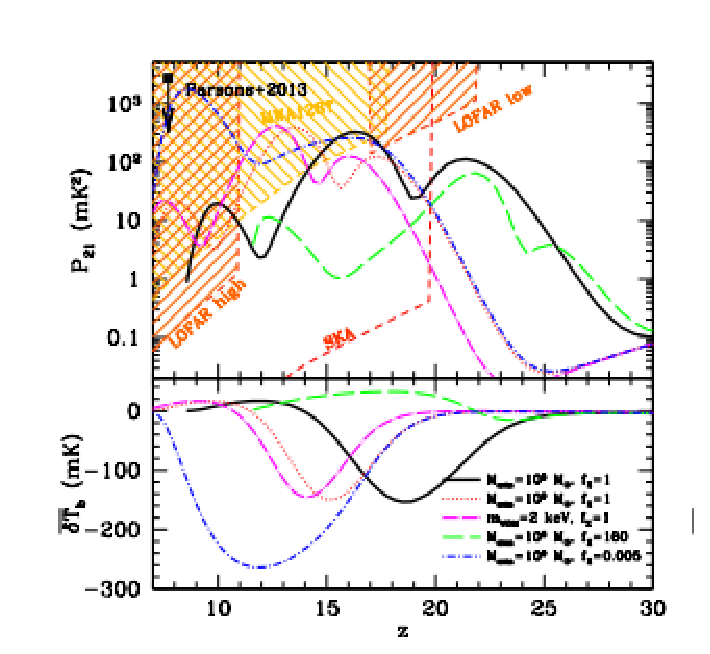
\includegraphics[width=0.5\hsize]{EoR/c03/c03.s2.f15.eps}
% \caption{(top)$z$$B$N4X?t$H$7$F8+$?;~$N(B21cm$B%Q%o!<%9%Z%/%H%k(B(fiducial model$B$O9u@~(B)$B$H(BMWA, LOFAR, SKA$B$N%N%$%:6J@~!#(B(bottom)$B51EY29EY$N(B$z$$B?J2=!#(B}
% \label{bukuro.constraining.fig:fig1}
% \end{figure}

\subsubsection{$B=i4|6d2O$N(BX$B@~J|<M$N@-<A(B}
$B=iBe6d2O$+$i$N(BX$B@~J|<M$O(BIGM$B$N29EY$r(BCMB$B29EY$h$j$b9b$$29EY$^$G>e>:$5$;$k$b(B
$B$N$H9M$($i$l$F$*$j!"(BIGM$B$N%$%*%s2=3d9g$,?t(B$\%$$BDxEY$N$H$-!"(BX$B@~J|<M$N%(%M%k(B
$B%.!<$N$[$H$s$I$,(BIGM$B$N2CG.$K$D$.9~$^$l$k!#(BX$B@~J|<M$O%$%*%s2=$h$j$b2CG.8;$H(B
$B$7$F8z2LE*$G$"$k!#$7$+$7!"4V@\E*$K$O$G$O$"$k$,!"(BX$B@~J|<M$K$h$C$F%8!<%s%:(B
$B<ANL$,>e$,$j!"8w;R2CG.$N%U%#!<%I%P%C%/$,CY$l$k$3$H$K$h$C$F:FEEN%$rCY$i$;(B
$B$k$H$$$&8z2L$b$"$k(B \citep{2013MNRAS.431..621M}$B!#(BX$B@~J|<M$H(BIGM$B$NAj8_:nMQ$O(B
$B$=$NBg$-$JJ?6Q<+M39TDx$K$h$C$FFCD'IU$1$i$l$k!J<0(B.\ref{eq:mfp}$B!K!#(B 
\begin{equation}
\lambda_{X}\sim 20 \overline{x}_{{\rm HI}}^{-1}\left(\frac{E_{X}}{300{\rm eV}}\right)^{2.6}\left(\frac{1+z}{10}\right)^{-1}c{\rm Mpc}
\label{eq:mfp}
\end{equation}
$\overline{x}_{{\rm HI}}$$B$OJ?6QCf@-?eAGN($G$"$j!"(B$E_{X}$$B$O8w;R$N%(%M%k%.!<(B
$B$G$"$k!#$3$N<0$h$j!"Fp(BX$B@~J|<M(B($E_{X}\le {\rm keV}$)$B$,(BIGM$B$HAj8_:nMQ$7!"(B
21cm$B@~$N8&5f$H7k$S$D$/;v$,J,$+$k!#(BIGM$B$N2CG.$K$h$k1F6A$O(B21cm$B%Q%o!<%9%Z%/(B
$B%H%k$N#2$DL\$N%T!<%/$KI=$l$k$,!"(BSKA1$B$G$O$3$N;~4|$N(B21cm$B%Q%o!<%9%Z%/%H%k$O(B
$B4QB,2DG=$HM=A[$5$l$F$$$k(B($B?^(B\ref{KH4})$B!#(B
%$B?^(B\ref{bukuro.constraining.fig:fig1}$B!K(B 

\subsubsection{$B2CG.4|$N(B21cm forest}
IGM$B$N29EY$,(BCMB$B29EY$h$j$b9b29$K2CG.$5$l$k0JA0$K$O!"9b@VJ}JP0\$NGX7JEEGH8;(B
$B$+$i$N8w$r(BIGM$B$,5[<}$9$k$3$H$K$h$j!"(B21 cm$B5[<}@~$,4QB,$5$l$k!#$3$l$r(B
Ly$\alpha$ forest$B$H$N%"%J%m%8!<$G(B21 cm forest$B$H8F$V!#(BSKA$B$G$b$3$N(B21 cm
forest$B$r4QB,$G$-$k$+$OFq$7$$$H$5$l$F$$$k(B \citep{2012MNRAS.425.2988M}$B!#:G(B
$BBg$NLdBj$H$7$F5s$2$i$l$k$N$OEEGH$r6/$/H/$9$k%/%'!<%5!<$J$I$NGX7JEEGH8;$,(B
$B9b@VJ}JP0\$G$bB8:_$9$k$+$H$$$&$3$H$G$"$k!#$7$+$7!"0E$$%/%'!<%5!<$G$bE}7W(B
$BE*<jK!$rMQ$$$l$P!"(B21cm forest$B$N8z2L$r2CG.4|A0$N(B21cm$B%Q%o!<%9%Z%/%H%k$N>.(B
$B%9%1!<%k$G8+$i$l$k2DG=@-$,$"$k(B \citep{2014MNRAS.441.2476E}$B!#(B21 cm$B%Q%o!<%9(B
$B%Z%/%H%k$NBg%9%1!<%k$O(BX$B@~$rJ|<M$9$k6d2O$K$h$k29EYMI$i$.$,;YG[E*$G$"$k$,!"(B
$B>.%9%1!<%k$G$O9b@VJ}JP0\$NEEGH$r6/$/H/$9$k(BAGN$B$J$I$,8z$$$F$/$k$N$G!"9b@V(B
$BJ}JP0\$N(BAGN$B$N<oB2$X$N@)8B$J$I$,4|BT$5$l$F$$$k!#(B 

\subsubsection{EoR$B%=!<%9(B}
EoR$B$N;~4|$d4|4V$NB>$K!"(B21cm$B%7%0%J%k$O(BEoR$B%=!<%9<+BN$K$D$$$F$b8@5Z$G$-$k!#(B
EoR$B$O8=:_$N4QB,$d>-Mh4QB,$N46EY8B3&$r2<2s$kbd>.6d2O$K$h$C$F0z$-5/$3$5$l(B
$B$k$H9M$($i$l$F$$$k$,!"$3$N$h$&$J9b@VJ}JP0\$Nbd>.6d2OFb$G$N@17A@.8zN($OITDj(B
$B@-$,Bg$-$/!"%U%#!<%I%P%C%/2aDx$b$h$/J,$+$C$F$$$J$$!#$7$+$7!"%U%#!<%I%P%C(B
$B%/8z2L$,@17A@.8zN($N?J2=$rD4@0$9$k$H9M$($i$l$F$*$j!"%U%#!<%I%P%C%/$NMM;R(B
$B$rCN$k;v$O(BEoR$B%=!<%9$rCN$k>e$G=EMW$G$"$k!#$3$l$rCN$k<j$,$+$j$N0l$D$H$7$F(B
EoR$B$N4v2?3XE*FCD'$r4QB,$9$k$H$$$&J}K!$,$"$k!#%$%*%s2=$r5/$3$7$F$$$k9=B$(B
$B$h$j$b>.%9%1!<%k$N(BEoR$B$N4v2?3XE*FCD'$r4QB,$9$k;v$K$h$j!"(BEoR $B%=!<%9$,$I$N(B
$B$h$&$K%O%m!<$H7k$S$D$-!"@17A@.8zN($K1F6A$rM?$($k$N$+$rCN$k;v$,$G$-$k$H9M(B
$B$($i$l$k!#(B 
%HIデータを用いたCDとEoRへの制限
\subsection{$B%P%j%*%s$H%@!<%/%^%?!<$NAjBPB.EY(B} 
\label{c03.s2.ss8}

$B1'Ch$N@2$l>e$,$j0J9_$N%P%j%*%s$NL)EY$f$i$.$N;~4VH/E8$dG.;K$O!"=iBeE7BN(B
$B!J=iBe@1!&=iBe6d2O!K7A@.2aDx$K$*$$$F=EMW$JLr3d$r2L$?$9!#FC$K!"=iBeE7BN$+(B
$B$i$NmU<M$O!"1'Ch$N:FEEN%$r5/$3$71'Ch0E9u;~Be$d$=$N8e$NE7BN7A@.$KBg$-$J1F(B
$B6A$rM?$($k$?$a!"1'Ch@2$l>e$,$j0J9_$N9=B$7A@.$rM}O@E*$KM}2r$9$k$3$H$O6K$a(B
$B$F=EMW$G$"$k!#(B

$B6aG/!"1'Ch@2$l>e$,$j0J9_$K$*$1$k%P%j%*%s$H%@!<%/%^%?!<$NAjBPB.EY$,9=B$7A(B
$B@.$dE7BN7A@.$KM?$($k1F6A$,(B\citet{2010PhRvD..82h3520T}$B$K$h$C$F;XE&$5$lCmL\(B
$B$r=8$a$F$$$k!#E57?E*$JAjBPB.EY$OFs>hJ?6Q$G(B30km/s$BDxEY$H$J$j!"@2$l>e$,$jD>(B
$B8e$N2;B.(B(6km/s)$B$rBg$-$/>e2s$kD62;B.$JAjBPB.EY$,IaJWE*$KB8:_$9$k!#$3$l$^$G(B
$B$NM}O@E*$J8&5f$G$O!"%P%j%*%s$H%@!<%/%^%?!<$NAjBPB.EY$K$h$k9=B$7A@.$KBP$9(B
$B$k1F6A$O#2<!$N8z2L$G$"$j!"$"$^$jCmL\$5$l$FMh$J$+$C$?$,!"%P%j%*%s$H%@!<%/(B
$B%^%?!<$K$3$N$h$&$JBg$-$JAjBPB.EY$,B8:_$9$k>u67$G$O!"=i4|$KAjBPB.EY$,$J$$(B
$B>l9g$HHf3S$7$F%@!<%/%^%?!<%O%m!<$N?tL)EY$d$=$NFbIt$N%P%j%*%s%U%i%/%7%g%s(B
$B$,>.$5$/$J$k$3$H$,(B\citet{2012ApJ...747..128N, 2013ApJ...763...27N}$B$N8&5f(B
$B$GL@$i$+$H$J$j!"%P%j%*%s$H%@!<%/%^%?!<$NAjBPB.EY$K$h$kE7BN7A@.$KBP$9$k1F(B
$B6A$K$D$$$F$N8&5f$,(B2010$BG/0J9_$K@9$s$K$J$C$F$-$F$$$k!#(B


$B%P%j%*%s$H%@!<%/%^%?!<$NAjBPB.EY$K$h$C$F1F6A$r<u$1$k%@!<%/%^%?!<%O%m!<$N(B
$B<ANL%9%1!<%k$O$=$N;~!9$N(BJeans$BD9$d(BJeans$B<ANL$N;~4VJ?6Q$KAjEv$9$k(B
filtering mass$B$N%9%1!<%k$G$"$j!"6qBNE*$K$O<g$K(B$10^5M_{\odot}$$B!A(B
$10^7M_{\odot}$$B$N%@!<%/%^%?!<%O%m!<$N7A@.$K1F6A$,=P$k!#$3$N%9%1!<%k$N%@!<(B
$B%/%^%?!<%O%m!<$O=iBe@1$d=iBe6d2O$KBP1~$7!"AjBPB.EY$N%3%R!<%l%s%9%9%1!<%k(B
$B$O%P%j%*%s2;6A?6F0$N%9%1!<%k(B($108h^{-1}$Mpc)$B$H$[$\F1$8$G$"$k$?$a!"1'Ch:F(B
$BEEN%4|$*$1$kE7BN7A@.$d:FEEN%$=$N$b$N$KBP$7$FBg$-$J%$%s%Q%/%H$rM?$($k$HM=(B
$BA[$5$l!"I,A3E*$K(BSKA$B$K$h$kCf@-?eAG(B21cm$B@~$N4QB,$,%P%j%*%s$H%@!<%/%^%?!<$NAj(B
$BBPB.EY$,E7BN7A@.$K5Z$\$91F6A$K$D$$$F$NCN8+$rF@$k6/NO$J<jCJ$H$J$k!#(B

$B1'ChO@E*$J9=B$7A@.$N?tCM%7%_%e%l!<%7%g%s$rMQ$$$F!"%P%j%*%s$H%@!<%/%^%?!<(B
$B$NAjBPB.EY$,:FEEN%4|$NE7BN7A@.$K5Z$\$91F6A$rD4$Y$k8&5f$,J#?t$N8&5f%0%k!<(B
$B%W$G9T$o$l$F$$$k(B
\citep{2011MNRAS.412L..40M,2012ApJ...747..128N,2013ApJ...763...27N}$B!#?^(B
\ref{c6.s3.ss5.f1}$B$O@VJ}JP0\(B$23$$B$H(B$19$$B$K$*$$$F7A@.$5$l$?%,%9%/%i%&%I$N<ANL4X(B
$B?t$r<($7$?$b$N$G!"B.EY:9$N1F6A$H$7$F%,%9%/%i%&%I$N<ANL$H?tL)EY$,2<$,$k79(B
$B8~$,L@3N$K$o$+$k!#B.EY:9$,(B$60$ km/s$B$N>l9g$N%,%9%/%i%&%I$N<ANL4X?t$O!"(B
$\sigma_8$$B$r(B$0.9$$B$+$i(B$0.8$$B$K2<$2$?>l9g$HF1DxEY$N1F6A$,$"$k!#;~4V$,7P$D$H!"B.(B
$BEY:9$,>.$5$/$J$k$?$a$KB.EY:9$NM-L5$K$h$k<ANL4X?t$X$N1F6A$O>.$5$/$J$k798~(B
$B$,8+$i$l$k!#@VJ}JP0\(B$19$$B$K$*$$$F$O!"B.EY:9$NM-L5$K$h$C$F<ANL4X?t$K(B2$BG\DxEY$N(B
$B0c$$$,8+$i$l$?$,!"@VJ}JP0\(B$10$$B$G$OB.EY:9$NM-L5$K$h$k<ANL4X?t$X$N1F6A$O$h$j(B
$B8BDjE*$H$J$j(B$10$\%$BDxEY$H$J$k!#$^$?!"0lC6%,%9%/%i%&%IFb$G$N@17A@.$,;O$^$k$H!"(B
$BAjBPB.EY$N1F6A$O7A@.$5$l$k=iBeE7BN$N7A@.N(!&EEN%8w;R$K$h$k:FEEN%!&=E85AG(B
$B6!5k$J$I$KGH5Z$9$k!#AjBPB.EY$NBg$-$JNN0h$G$O!"@17A@.N($N?d0\$,B>$NNN0h$h(B
$B$j$bCY1d$7!"$=$l$KH<$C$F:FEEN%$d=E85AG6!5k$bCY1d$9$k(B($B?^(B
\ref{c6.s3.ss5.f2})$B!#$3$N7k2L!"AjBPB.EY>l$N%3%R!<%l%s%9%9%1!<%k$GEEN%EY$N(B
$B6u4VE*JQF0$,H/@8$7!"(B21 cm$B@~J|<M$N6u4VJ,I[$N%Q%o!<%9%Z%/%H%k$KH?1G$5$l$k$H(B
$BM=A[$5$l$k!#(B

\begin{figure}[!t]
 \centering \includegraphics[width=0.9\linewidth] {EoR/c03/c03.s2.f16.eps}
 \caption{$B@VJ}JP0\(B23($B>eCJ(B)$B$H(B19($B2<CJ(B)$B$K$*$1$k%,%91@$N<ANL4X?t!#:8$H1&$O$=(B
 $B$l$>$l(Bdifferential$B$J<ANL4X?t$H(Bcumulative$B$J<ANL4X?t!#(B
 \label{c6.s3.ss5.f1}}
\end{figure}
\begin{figure}[!h]
 \centering \includegraphics[width=10cm] {EoR/c03/c03.s2.f17.eps}
 \caption{$B>eCJ!'%P%j%*%s$H%@!<%/%^%?!<$NAjBPB.EY$NBP$9$k(BPop-III$B$HA4BN$N@1(B
 $B7A;K$N;~4VH/E8!#2<CJ!'(BPop-III$B$N7A@.N($NA4BN$N@17A@.N($KBP$9$k4sM?$N;~4VH/E8!#(B
 \label{c6.s3.ss5.f2}}
\end{figure}


SKA$B$N4QB,7k2L$r@5$7$/2r<a$9$k$K$O!"%P%j%*%s$H%@!<%/%^%?!<$NAjBPB.EY$K$h$k(B
$B9=B$7A@.$X$N1F6A$rDjNLE*$K8+@Q$b$k$3$H$,I,MW$G$"$k!#@VJ}JP0\$,(B$20$$B0J>e$N@1(B
$B7A@.3hF0$,;O$^$C$F$$$J$$;~4|$N4QB,$K$O!"%,%9%/%i%&%I$KK-IY$K4^$^$l$k(B
H$_2$$B$d(BHD$B$H$$$C$?J,;R$N2sE>A+0\J|<M$,%,%9$NJ,I[$NNI$$%H%l!<%5!<$H$J$k!#(B
H$_2$$B$N(B$J=2\rightarrow 0$$B$N2sE>A+0\!"(BHD$B$N(B$J=4\rightarrow 3$$B$N2sE>A+0\$,=P(B
$B$9(B$533$ GHz$B$NJ|<M$O@VJ}JP0\(B$35\sim 40$$B$G$"$l$P!"(B$14$ GHz$B$^$G4QB,$G$-$k(BPhase-1$B$N(B
SKA-MID $B$G4QB,2DG=$G$"$k!#99$K(B $24$ GHz$B$^$G4QB,2DG=$G$"$k(BPhase-2$B$G$"$l$P!"@V(B
$BJ}JP0\(B$20$$BDxEY$^$G4QB,2DG=$G$"$k!#$^$?!"=iBeE7BN$,7A@.$5$l1'Ch:FEEN%$,?J$`(B
$B2aDx$G$N%P%j%*%s$H%@!<%/%^%?!<$NAjBPB.EY$N1F6A$r4QB,$9$k$K$O!"Cf@-?eAG$N(B
21 cm$B@~$r%H%l!<%5!<$H$7$F@VJ}JP0\(B$6<z<20$$B$NCf@-?eAG$+$i$NJ|<M$r(B$50 \sim 350$
MHz
$B$N<~GH?tBS$r%+%P!<$9$k(BSKA-low$B$,:GE,$G$"$k!#(B

%バリオンとダークマターの相対速度
\subsection{EoR/Cosmic Dawn$B4|$N1'ChO@(B}
\label{c03.s2.ss9}

$B6aG/!"(BWMAP, Planck$B$r$O$8$a$H$9$k1'Ch%^%$%/%mGHGX7JmU<M(B(CMB)$B29EYMI$i$.$dJP(B
$B8w$N4QB,!"$^$?(BSDSS$B$r$O$8$a$H$9$kBg5,LO6d2O%5!<%Y%$$K$h$k!"1'Ch$N9=@.MWAG(B
$B$dMI$i$.$N=i4|>r7o$rM?$($k%$%s%U%l!<%7%g%sM}O@$r5-=R$9$k1'ChO@%Q%i%a!<%?(B
$B$N@:L)B,Dj$,2DG=$H$J$j!"1'ChO@$O@:L)2J3X$H$7$F3NN)$5$l$F$-$F$$$k!#(B

$B$7$+$7$^$@$^$@!"%@!<%/%^%?!<!"%@!<%/%(%M%k%.!<$N@5BN$d%K%e!<%H%j%N<ANL$J(B
$B$I2r7h$9$Y$-LdBj$,B8:_$9$k!#>-Mh4QB,$K$*$1$k$3$l$i$NLdBj2r7h$KBP$9$k%"%W(B
$B%m!<%A$H$7$F$O!"C1=c$K$O;~4V!"6u4VE*$K$h$jI}9-$$4QB,$r9T$&$3$H$G$"$k!#(B

SKA$B$O!"0J>e$N$h$&$J8=:_$N1'ChO@$K$*$1$kLdBj2r7h$K$H$C$FHs>o$K=EMW$J0LCV$r(B
$B@j$a$F$$$k!#$3$l$^$G4QB,$7$?$3$H$N$J$$!";~4VE*$K$O9b@VJ}JP0\1'Ch$N>pJs$r(B
$BM?$($F$/$l$k$@$m$&$7!"6u4VE*$K$O$h$j>.$5$J%9%1!<%k$^$G4QB,$G$-$k$+$i$G$"(B
$B$k!#(B

\paragraph{$BL)EYMI$i$.$N>pJs$rMQ$$$?1'ChO@%Q%i%a!<%?$X$N@)8B(B}

SKA$B$O!"(B21cm$B51EY29EY!J(B21cm$B%7%0%J%k!K$rL)EY>l$NDI@W;R!J%H%l!<%5!<!K$H$7$F;H$$!"(B
$B1'ChO@%Q%i%a!<%?$KBP$7$F@)8B$rM?$($k$3$H$,=PMh$k!#(B

$B$3$N51EY29EY$O!"%9%T%s29EY!"Cf@-?eAG$N3d9g$HL)EY>l$K0MB8$9$k!#(B
$BFC$K%9%T%s29EY$,(BCMB$B29EY$KHf$Y$FHs>o$K9b$$>l9g!"(BCMB$B29EY$+$i$_$?51EY29EY$O!"(B
$B$*$*$h$=(B
\begin{equation}
\delta T_B = (1 + \delta ) x_H \times \cdots
\end{equation}
$B$H=q$1$k!#(B$x_H$$B$,Cf@-?eAG$N3d9g$G!"(B$\delta$$B$,J*<A$NL)EY>l$rI=(B
$B$9(B~\citep{2006PhR...433..181F}$B!#FC$K(B$x_H = 1$$B$N>l9g$K$O(B$\delta T_B$$B$O!"L)(B
$BEY>l$NL5%P%$%"%9DI@W;R$H$J$k!#$3$N$h$&$JHs>o$KM}A[2=$5$l$?>u67$G$N%Q%i%a!<(B
$B%?7hDj@:EY$O!"(BSKA0 (SKA1$B$NH>J,$N%"%s%F%J$N?t(B)$B$G(B$z=7,7.5,8$$B$G$N51EY29EY$r(B
$B4QB,$7$?>l9g!"(BPlanck$B$H$[$\F1DxEY!"(BSKA2(SKA1$B$N#4G\$N%"%s%F%J$N?t(B)$B$G$O!"FC(B
$B$K>.%9%1!<%k$N>pJs$r$h$j@:L)$KB,Dj$9$k$3$H$,2DG=$H$J$k$N$G!"Nc$($P=i4|MI(B
$B$i$.%Q%o!<%9%Z%/%H%k$N%9%Z%/%H%k;X?t$NJQ2=(B(running spectral index)$B$d%K%e!<(B
$B%H%j%N<ANL$N7hDj@:EY$,(BPlanck$B$KHf$Y%U%!%/%?!<#3DxEY2~A1$9(B
$B$k(B~\citep{2008PhRvD..78f5009P,2009PhLB..673..173B, 2011JCAP...02..021A}$B!#(B

\paragraph{$B!V1'ChO@E*MWAG!W$H!V1'ChJ*M}E*MWAG!W$NJ,N%(B}

$B$7$+$7<B:]$K$O!"$3$N$h$&$JM}A[E*$J>u67$K$O$J$C$F$*$i$:!"4QB,$5$l$k@VJ}JP(B
$B0\$G$N%,%929EY$J$I$5$^$6$^$J1'ChJ*M}E*$JMWAG$,(B$\delta T_B$$B$K$O:.F~$7$F$/(B
$B$k!#1'ChO@$H$3$N1'ChJ*M}E*$JMWAG$r40A4$KJ,N%$9$k$?$a$K$O!"1'ChJ*M}E*8z2L(B
$B$KBP$9$kM}O@%b%G%k$N9=C[$,$^$:9M$($i$l$k(B~\citep{2008PhRvD..78b3529M}$B!#$b$&(B
$B$R$H$D$O!"(B$\delta T_B$$B$N%Q%o!<%9%Z%/%H%k$K$*$1$k@VJ}JP0\OD$_$rMQ$$$k$3$H(B
$B$G$"$k!#$3$N@VJ}JP0\OD$_$O!"%I%C%W%i!<%7%U%H$K5/0x$9$k$,4QB,E*$K$O%Q%o!<(B
$B%9%Z%/%H%k$r3QEY0MB8@-$GE83+$7$?:]$K9b<!%b!<%a%s%H$H$7$FM?$($i$l$k!#FC$K(B
$B%X%-%5%G%+%]!<%k$O1'ChJ*M}E*8z2L$,F~$i$J$$L)EY>l$N$h$$DI@W;R$H$7$F9M$($i(B
$B$l!"$3$N9b<!%b!<%a%s%H$N4QB,$b=EMW$H9M$($i$l$k(B~\citep{2006ApJ...653..815M,2008PhRvD..78b3529M}$B!#(B

\paragraph{$B6d2O4V%,%929EY$N>pJs$rMQ$$$??7J*M}$NC5::(B}

$BL)EY>l$NDI@W;R$H$7$F>e$G$O(B21cm$B%7%0%J%k$r9M$($F$-$?$,!"@h$K$b=R$Y$?$h$&$K(B
21 cm$B%7%0%J%k$O!"1'Ch$N%$%*%s2=N($d6d2O4V%,%9(B(inter galactic medium
(IGM))$B$N29EY$K$b0MB8$9$k!#I8=`1'Ch%b%G%k$K$*$1$k9=B$7A@.%7%J%j%*$K4p$E$$(B
$B$?!"%$%*%s2=N($d(BIGM$B$N>uBV$N;~4VJQ2=$K2C$($F!"$5$i$K$3$l$i$N?J2=$,JQ99$r<u(B
$B$1$k$h$&$J?7$?$J%7%J%j%*$,$"$l$P!"(B21 cm$B%7%0%J%k$N4QB,$O9b@VJ}JP0\1'Ch$K$*(B
$B$1$k?7$?$JJ*M}$X$N@)8B$rM?$($k$b$N$H$7$F=EMW$G$"$k!#(B

$B$^$:$=$N$h$&$J8uJd$H$7$F!"0E9uJ*<A$N@-<A$,>e$2$i$l$k!#I8=`E*$JNd$?$$0E9u(B
$BJ*<A!J(BCDM$B!K%b%G%k$H$O0[$J$j!"<ANL$,Hf3SE*7Z$$$h$&$J$$$o$f$kCH$+$$0E9uJ*<A(B
 (Warm Dark Matter(WDM)) $B$,$7$P$7$P5DO@$5$l$F$$$k!#$3$N(BWDM$B%b%G%k$G$O!">.%9(B
$B%1!<%k9=B$$N7A@.$,M^@)$5$l!"6d2O7A@.$,I8=`E*$JNd$?$$0E9uJ*<A$N>l9g$h$jCY(B
$B$/$J$k!#7k2L$H$7$F!"(B21 cm$B%7%0%J%k$K$*$$$F!"1'ChJ*M}E*MWAG$,1F6A$rM?$($k;~(B
$B4|$,JQ99$r<u$1$k$N$G4QB,$+$i$3$N(BWDM$B%7%J%j%*$K@)8B$rM?$($k$3$H$,$G$-$k$H4|(B
$BBT$5$l$k(B~\citep{2014MNRAS.438.2664S}$B!#(B


$B$^$?0E9uJ*<A$NBP>CLG$dJx2u$r9M$($k$H!"$=$l$O(BIGM$B$rCH$a$k8z2L$H$7$FF/$-!"(B
IGM$B29EY$N;~4V?J2=$NMM;R$,I8=`%b%G%k$H$O0[$J$C$F$/$k!#$3$N$h$&$J(BIGM$B29EY$N(B
$B;~4VJQ2=$rDL$8$??7$?$J%b%G%k$X$N@)8B$K$H$C$F$b(B21cm$B%7%0%J%k$OM-8z$G$"(B
$B$k(B~\citep{2014JCAP...11..024E}$B!#(B

$BB>$K$b!"=i4|<'>l$d!"86;O%V%i%C%/%[!<%k$J$I$N!VJQ$o$C$?FC@-$r;}$C$?J*<A!W(B
$B$KBP$9$k@)8B$H$7$F$b(BSKA$B$K$h$k(B21cm$B4QB,$O=EMW$G$"$k$H9M$($i$l(B
$B$k(B~\citep{2014PhRvD..89j3522S}$B!#(B 

\paragraph{$B%P%k%/%U%m!<(B}

$B>\:Y$O(B``Bulk flows and the end of dark ages''$B$G?($l$k$,!"(Bbaryon$B$H0E9uJ*<A(B
$B$N4V$NB.EY>l$N0c$$$,9=B$7A@.$K1F6A$rM?$($k$3$H$,!";XE&$5$l$F$$(B
$B$k(B~\citep{2010PhRvD..82h3520T}$B!#$3$NAjBPB.EY$N1F6A$H$7$F$O!">.%9%1!<%k$N9=(B
$BB$7A@.$NM^@)$J$I$,9M$($i$l$k!#$3$N8z2L$O!"(B21 cm$B%7%0%J%k$GC5$k9b@VJ}JP0\1'(B
$BCh$G82Cx$G$"$k$N$G!"(BSKA$B$GC5$k?7$?$J1'ChO@E*8z2L$H$7$F5DO@$5$l$F$$$k!#(B


\paragraph{$B$=$NB>(B}

\begin{itemize}

\item $B=i4|Hs%,%&%9@-(B

$B=i4|6JN(MI$i$.$NE}7WJ,I[$O!"MI$i$.$N<o$H$J$k%9%+%i!<>l$NAj8_:nMQ$d>l$NMI$i$.$r6JN(MI$i$.$X$HE>49$9$k:]$NHs@~7A8z2L$K$h$j%,%&%9J,I[$+$i$o$:$+$K$:$l$k2DG=@-$,$"$k$3$H$,;XE&$5$l$F$$$k!#$3$N$h$&$J>l9g!"Hs>o$KBg$-$J%9%1!<%k$G$N6d2OJ,I[$,1F6A$r<u$1$F(B
$B%,%&%9J,I[$N;~$H$O0[$J$k%Q%o!<%9%Z%/%H%k$N?6$kIq$$$,8+$i$l$k!#1'Ch:FEEN%4|$N(B21cm$B%7%0%J%k$K$O!"(B
$B%$%*%s2=N($N>pJs$,F~$C$F$$$k$,!"$3$N%$%*%s2=N($,6u4VJ,I[$7$F$$$k>l9g!"(B21cm$B51EY29EY$N%Q%o!<%9%Z%/%H%k$O!"$=$NJ,I[$K0MB8$9$k!#6d2OJ,I[$HF1$8$h$&$K!"$3$N%$%*%s2=N($NJ,I[$K$b=i4|MI$i$.$NHs%,%&%9@-$O1F6A$rM?$($k$N$G!"(BSKA$B$J$I$K$h$j=i4|MI$i$.$NHs%,%&%9@-$K@)8B$rM?$($k$3$H$,=PMh$k!#(B
Planck$B$K$h$k(BCMB$B4QB,$GF@$i$l$F$$$k$3$NHs%,%&%9@-$KBP$9$k@)8B$HF1DxEY$N@)8B$rM?$($k$H4|BT$5$l$F$$$k(B~\citep{2011PhRvL.107m1304J}$B!#(B


\item $B1'ChO@E*=ENO%l%s%:8z2L(B

$B9b@VJ}JP0\$GH/$;$i$l$?(B21cm$B%7%0%J%k$O2f!9$KFO$/$^$G$K1'ChBg5,LO9=B$$rDL2a$7$F$/$k$N$G$=$N=ENO>l$N1F6A$K$h$C$F%l%s%:8z2L$r<u$1$k!#$3$N%l%s%:8z2L$rCj=P$G$-$l$P!"$"$i$?$J1'ChBg5,LO9=B$$N(Bprobe$B$H$7$F4|BT$G$-$k!#(BSKA$B$G$O==J,B,Dj2DG=$G$"$k$H9M$($i$l$F$$$k(B~\citep{2006ApJ...653..922Z,2006astro.ph.11862B}$B!#(B

\end{itemize}

\paragraph{$B$^$H$a(B}

SKA$B!J(BSKA-Low$B!K$O!"@VJ}JP0\$r<u$1$?Cf@-?eAG$N(B21cm$B@~%7%0%J%k$rB*$($k$3$H$G(B
$z = 6 - 27$$B$H$$$&9b@VJ}JP0\1'Ch$N;Q$rL@$i$+$K$9$k$H4|BT$5$l$F$$$k!#$3$N4QB,$K$h$j!"$3$l$^$G$N1'ChO@%Q%i%a!<%?$N7hDj@:EY$,8~>e$9$k$@$1$G$J$/!"0E9uJ*<A$N@-<A$J$I?7$?$JJ*M}$K4QB,E*$KGw$k$3$H$,$G$-$k$H4|BT$5$l$F$$$k!#(B


%Cosmology from EoR/Cosmic Dawn
\subsection{$B1'ChO@E*4QB,$HCf@-?eAG(B21~cm$B@~$NAj8_Aj4X(B}%\label{c6.s2}
\label{c03.s2.ss10}

SKA$B7W2h$K$*$$$F!"(BCosmic Dawn~(CD)$B$d(BEpoch of Reionization~(EoR)$B5/8;$N1'Ch(B
$BO@E*$JCf@-?eAG(B21~cm$B@~$N8!=P$O=EMW$J%-!<%5%$%(%s%9$N0l$D$G$"$k!#$7$+$7$J$,(B
$B$i!"$=$N4QB,GHD9BS$OE7$N@n6d2O$d6aK56d2O$K$"$k6/$$EEGH8;!"CO5e$NEEN%AX$N(B
$B1F6A!"$=$7$F%i%8%*GH$N43>D$J$I$K$h$j7h$7$FM}A[E*$J4QB,>r7o$H$O8@$($J$$!#(B
$B$9$J$o$A!"1'ChO@E*(B21~cm$B$N%7%0%J%k$O$3$l$i(B''$B%N%$%:(B''$B$KKd$b$l$F$7$^$$!"$=$N(B
$B8!=P$O:$Fq$r6K$a$k!#$3$N$h$&$J:$Fq$5$r2sHr$9$kJ}K!$N0l$D$H$7$F!"B>$N4QB,(B
$B$H$NAj8_Aj4X$,5s$2$i$l$k!#Fs$D$NFHN)$J4QB,!J$b$7$/$OGHD9!K$NAj8_Aj4X$r$H(B
$B$l$P!"$=$l$>$l$N%7%9%F%^%F%#%C%/$J%N%$%:$O$*8_$$BG$A>C$79g$$!"%N%$%:$KKd(B
$B$b$l$F$$$?%7%0%J%k$N8!=P$,2DG=$H$J$k!#(B

CD$B$d(BEoR$B5/8;$N%7%0%J%k$r<h$j=P$9;v$rL\E*$H$7$?;~!"1'ChO@E*(B21~cm$B@~$HAj8_Aj(B
$B4X$r<h$kM-NO$J4QB,$H$7$F!"1'Ch%^%$%/%mGHGX7JJ|<M(B~(CMB)$B!"9b@VJ}JP0\$N6d2O(B
$BC5::!"$=$7$F!"6a@V30@~GX7JJ|<M(B~(NIRB)$B$,5s$2$i$l$k!#$3$N>O$G$O!"$3$l$i$N4Q(B
$BB,$H(BCD$B$d(BEoR$B$H$N4XO"@-!"$=$7$F!"1'ChO@E*(B21~cm$B@~$HAj8_Aj4X$r$H$k;v$K$h$C$F!"(B
$B$I$N$h$&$J(BCD$B$d(BEoR$B$K4X$9$k>pJs$K%"%/%;%9=PMh$k$+$K$D$$$F%l%S%e!<$r$9$k!#(B

	
\subsubsection{CMB$B$H$NAj8_Aj4X(B}

CMB$B29EY$f$i$.$N@:L)4QB,$K$h$j!"2f!9$O1'Ch$NMM!9$J>pJs$K%"%/%;%9$G$-$k!#(B
$B$=$l$O!"1'Ch:F%$%*%s2=%W%m%;%9$bNc30$G$O$J$$!#(BCMB$B8w;R$O!"<+M3EE;R$H$N;6Mp$N:]!"(B
$B%I%C%W%i!<%7%U%H$r<u$1$k(B~\citep{zeldovich}$B!#(B
EoR$B4|$K$O<+M3EE;R?t$,G|Bg$KA}$($k$?$a!"$3(B
$B$N%I%C%W%i!<%7%U%H$,(BEoR$B4|5/8;$N29EY$f$i$.$,@8$8$k%a%+%K%:%`$H$J$k!#(B
$B$3$N;v$+$i!"(BCMB$B$N29EY$f$i$.$K$O!"(BEoR$B4|$N<+M3EE;R$N?tL)EY(B($B%$%*%s2=EY$b4^$`(B)$B$H$=$N!JG.1?F0$b$7$/$O%P%k%/1?F0$N!KB.EY$N?J2=;K$,Kd$a9~$^$l$F$$$k$H8@$($k!#(B
$BBg$^$+$K8@$($P!"Bg%9%1!<%k$N29EY$f$i$.$K$O1'ChJ?6Q$N%$%*%s2=EY$,!">.%9%1!<(B
$B%k$G$O%$%*%s2=%P%V%k$K$h$C$F:n$i$l$k6I=jE*$J%$%*%s2=EY$,$=$l$>$lL)@\$K4X(B
$B$o$C$F$/$k(B ($B>\$7$$%l%S%e!<$H$7$F!"Nc$($P(B~\cite{2008RPPh...71f6902A}
$B$r8+$h(B)$B!#(B

$B$7$+$7$J$,$i!"(BEoR$B4|$K@8@.$5$l$k29EY$f$i$.$O29EY$f$i$.A4BN$G8@$($P>.$5$/!"(B
$BB>$N5/8;$N29EY$f$i$.$N@.J,$KKd$b$l$F$$$k!#$3$NKd$b$l$?%7%0%J%k$rIb$+$S>e$,$i$;(B
$B$kJ}K!$N0l$D$,!"(B21~cm$B@~$H(BCMB$B$NAj8_Aj4X$G$"$k!#$7$?$,$C$F!"3F!9$N<+8JAj4X$G$OKd$b$l(B
$B$F$7$^$C$F$$$k(BEoR$B$N>pJs$K%"%/%;%9$G$-$k2DG=@-$b$"$k$3$H$+$i!"$3$NAj8_Aj(B
$B4X$NJ*M}$NM}2r$N$?$a$K!"2r@OE*!"?tCM7W;;E*$NN>J}$NLL$+$iB?$/$N8&5f$,$J$5(B
$B$l$F$$(B
$B$k(B~\citep{2005MNRAS.360.1063S,2008MNRAS.384..291A,2004PhRvD..70f3509C,2006ApJ...647..840A,2007MNRAS.377..168S,2010MNRAS.402.2617T,2010MNRAS.402.2279J,2011MNRAS.414.3424T}$B!#(B
$B$=$N7k2L!"Bg$-$J%9%1!<%k$G$NAj8_Aj4X%7%0%J%k$NBg$-$5$O!"1'ChJ?6QE*$J(B
$B%$%*%s2=$N%9%T!<%I$K0MB8$9$k$3$H$,<($5$l$?!#%$%*%s2=$,5^7c$K?J$`$[$I!"$=$N(B
$B%7%0%J%k$NBg$-$5$OBg$-$/$J$k$N$G$"$k!#?^(B~\ref{fig:cmb_cross}$B$O(B~\cite{2010MNRAS.402.2617T} $B$K4p$E$$$F!":F%$%*%s2=%b%G(B
$B%kKh$N(B
Signal-Noise ratio~(S/N)~$B$rI=$7$?$b$N$G$"$k!#2#<4$O4QB,$N(Bsky~fraction$B!"(B
$B=D<4$O(B21~cm$B@~4QB,$N5,3J2=$5$l$?%N%$%:%Q%o!<$G$"$k!#$3$N?^$G$O!"(BCMB$B29EY$f$i$.$N(B
$B4QB,$H$7$F!"(BPlanck$B1R@1$N46EY$r:NMQ$7$F$*$j!"1'Ch$NJ?6Q%$%*%s2=EY$N?J2=$N%b%G(B
$B%k$H$7$F!"(B
\begin{equation}
x_e(z) = \frac{1}{1+\exp[(z-z_{\rm re})/\Delta z]},
\end{equation}
$B$r:NMQ$7$F$$$k!#(B
$B$3$N%b%G%k$G$O!"(B$\Delta z$$B$,>.$5$$$[$I%$%*%s2=$,5^7c$K?J$`!#$=$N$?$a!"Aj8_Aj(B
$B4X$N%7%0%J%k$bBg$-$/$J$k$N$G!"(BS/N$B$O>.$5$$(B$\Delta z$$B$[$IBg$-$/$J$k!#(B
$B8=:_7W2h$5$l$F$$$k3F(BSKA$B$N%G%6%$%s$O@VE@$G<($5$l$F$$$k!#$7$?$,$C$F!"(BSKA$B$G$NAj8_Aj4X$N%7%0%J%k$N8!=P!"L$8!=P$K$h$j:F%$%*%s2=%W%m%;%9$K$D$$$F@)8B$rM?$($k2DG=@-$,$"(B
$B$k$3$H$,$o$+$k!#(B


\begin{figure}[!t]
 \begin{minipage}{0.5\hsize}
  \begin{center}
   \includegraphics[width=70mm]{EoR/c03/c03.s2.f18.eps}
  \end{center}
 \end{minipage}
 \begin{minipage}{0.5\hsize}
  \begin{center}
   \includegraphics[width=70mm]{EoR/c03/c03.s2.f19.eps}
  \end{center}
 \end{minipage}
  \caption{$B:F%$%*%s2=%b%G%kKh$N(B21~cm$B$H(BCMB$B$NAj8_Aj4X$N(BS/N$BHf!#2#<4$O(B21~cm$B@~4QB,$N(B
 sky~fraction$B!"=D<4$OB?=E6K(B$\ell =100$$B$G5,3J2=$5$l$?4QB,$N%N%$%:%Q(B
 $B%o!<(B~($B%N%$%:$N3QEY%Q%o!<%9%Z%/%H%k(B$N(\ell)$$B$O(B$N(\ell )
 =N_{100}(\ell/100)^2$$B$GM?$($i$l$k(B)$B!#:8%Q%M%k$G$O(B$\Delta z = 0.01$$B!#(B
 $B1&%Q%M%k$G$O(B$\Delta z = 0.1$$B!#N>%Q%M%k$H$b(B$z_{\rm re} = 10$$B$G$"$j!"4QB,(B
 $B<~GH?t$O(B$z=10$$B$KBP1~$9$k!#(B}
  \label{fig:cmb_cross}
\end{figure}




\subsubsection{$B9b@VJ}JP0\6d2O$H$NAj8_Aj4X(B}

$B6d2O$OL)EY$f$i$.$N%H%l!<%5!<$G$"$k$HF1;~$K!"M-NO$J1'Ch:F%$%*%s2=8;$N0l$D(B
$B$H$7$F9M$($i$l$F$$$k!#$=$N$?$a!"1'ChO@E*(B21~cm$B@~$N%7%0%J%k$N6/$5$H6d2O$N(B
$B?tL)EY$H$NAj8_Aj4X$O!"1'Ch$N%$%*%s2=EY$K1~$8$F!"$9$3$7J#;($JMMAj$r<($9(B~\citep{2009ApJ...690..252L,2013MNRAS.432.2615W}$B!#(B

\begin{figure}[!t]
  \begin{center}
   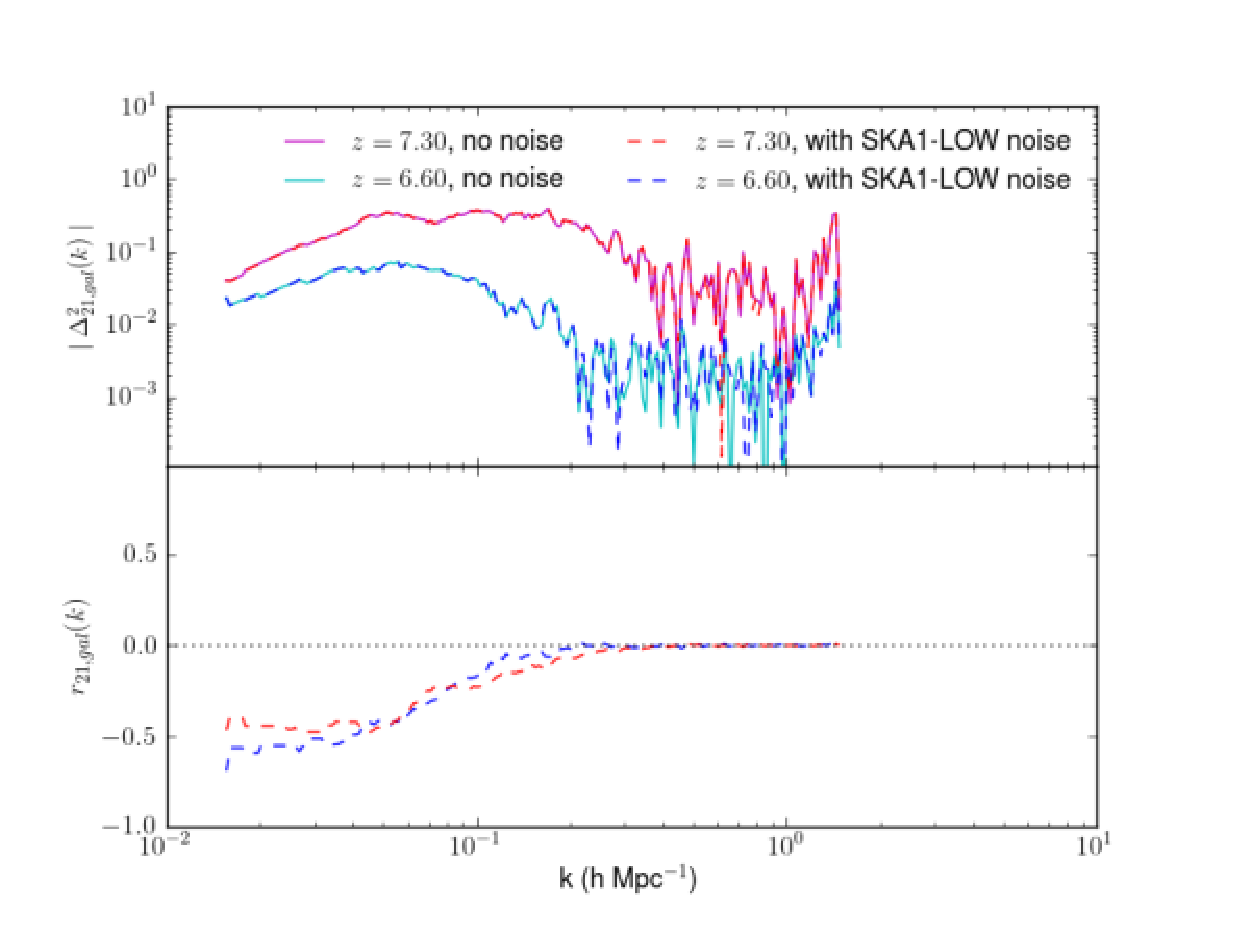
\includegraphics[width=100mm]{EoR/c03/c03.s2.f20.eps}
  \end{center}
 \caption{21~cm$B@~$H6d2O$NAj8_Aj4X$NL5<!852=$5$l$?%Q%o!<%9%Z%/%H%k!J>e%Q%M%k!K$H$=$NAj(B
 $B4X78?t!J2<%Q%M%k!K!#$3$3$GAj4X78?t(B$r$$B$O(B,$B6d2O$H(B21~cm$B@~$NL5<!85%Q%o!<%9%Z%/%H%k!"(B
 $\Delta^2(k)_{\rm halo}$$B$H(B$\Delta^2(k)_{21}$$B$rMQ$$$F!"(B
 $r=\Delta^2(k)_{21,\rm halo}/ \Delta^2(k)_{\rm halo} \Delta^2(k)_{21}$$B!#(B
 }
  \label{fig:galaxy_cross}
\end{figure}
\begin{figure}[!h]
 \begin{minipage}{0.5\hsize}
  \begin{center}
\includegraphics[width=70mm]{EoR/c03/c03.s2.f21.eps}
  \end{center}
 \end{minipage}
 \begin{minipage}{0.5\hsize}
  \begin{center}
   \includegraphics[width=70mm]{EoR/c03/c03.s2.f22.eps}
  \end{center}
 \end{minipage}
  \caption{$B6a@V30$H(B21~cm$BAj8_Aj4X78?t$X$N(BSKA$B$N46EY!J:8%Q%M%k!K$H%$%*%s2=(B
 $BN((B($B@VJ}JP0\(B)$B0MB8@-!J1&%Q%M%k!K!#(B}
  \label{fig:nirb_cross}
\end{figure}

$B1'Ch:F%$%*%s2=A0!"$b$7$/$O$=$N=i4|$K$O!"1'ChO@E*(B21~cm$B@~$N%7%0%J%k$NBg$-(B
$B$5$OL)EY$f$i$.$NBg$-$5$KHfNc$9$k!#6d2O$N?tL)EY$b$^$?L)EY$f$i$.$NBg$-$5$K(B
$BHfNc$9$k$?$a!"N><T$NAj8_Aj4X$O@5Aj4X$H$7$F8=$l$k!#(B
$B1'Ch$N:F%$%*%s2=$,?J$`$H!"1'ChO@E*(B21~cm$B@~$N%7%0%J%k$NBg$-$5$OCf@-?eAG$,(B
$B$I$l$[$I%$%*%s2=$5$l$:$K;D$5$l$F$$$k$+$K0MB8$9$k!#6d2O$O%$%*%s2=8w;R$N6!(B
$B5k8;$H$J$j$($k$N$G!"EvA3!"6d2O$N?tL)EY$,B?$$$H$3$m$G$O!"B?$/$N?eAG$,%$%*(B
$B%s2=$5$l$k$3$H$K$J$k!#$=$N$?$a!"%$%*%s2=$5$l$F$$$kNN0h!J%$%*%s2=%P%V%k!K$O!"(B21~cm$B@~$H6d2O(B
$B$NAj8_Aj4X$K$*$$$F$O!"Ii$NAj4X$H$7$F8=$l$k!#(B
$B$7$?$,$C$F!"Ii$NAj4X$N8=$l$k%9%1!<%k$N@VJ}JP0\$KBP$9$k?J2=$h$j!"%$%*%s2=%P%V(B
$B%k$N@.D9$r8+$k;v$,$G$-$k!#(B



$B?^(B~\ref{fig:galaxy_cross}$B$O:F%$%*%s2=$N%7%_%e%l!<%7%g%s$h$jF@$i$l$?(BEoR$B4|$NAj8_Aj(B
$B4X$N%Q%o!<%9%Z%/%H%k$r<($7$F$$$k(B~\citep{2013MNRAS.432.2615W}$B!#?^$N2<%Q%M(B
$B%k$r$_$k$H(B$z=9$$B$G(B$k \sim 0.3-0.4~h{\rm Mpc}^{-1}$$B$G8=$l$F$$$k(B
$BH?Aj4X$,:F%$%*%s2=$,?J$`$K$D$l$FBg$-$J%9%1!<%k$K0\F0$7$F$$$k!#(B
$B$7$?$,$C$F!"9b@VJ}JP0\6d2O$H(B21~cm$B@~$NAj8_Aj4X$r$H$l$P!"(B
$B$=$l$>$l$N@VJ}JP0\$G$NE57?E*$J%P%V%k%5%$%:$K%"%/%;%9$G$-$k2DG=@-$,$"$k;v(B
$B$,$o$+$k!#(B





\subsubsection{NIRB$B$H$NAj8_Aj4X(B}


$B1'Ch=i4|$N6d2O$d@1!9$O!"1'Ch:F%$%*%s2=$N$?$a$NM-8z$J%$%*%s2=8w;R6!5k8;$G(B
$B$"$k!#$7$?$,$C$F!"9b@VJ}JP0\$N@17A@.;K$rM}2r$9$k;v$O!"1'Ch:F%$%*%s2=;K$X$NM}2r$X$H$D$J$,$k!#(B
$B8=:_$N4QB,$K0M$l$P!"1'Ch$N:F%$%*%s2=$N$?$a$K$O8=:_4QB,$5$l$F$$$k6d2O$d@1!9(B
$B$h$j$b$5$i$KB?$/$N0E$/$F4QB,$5$l$F$$$J$$6d2O$d@1$,I,MW$G$"$k$3$H$,L@$i$+(B
$B$K$5$l$?!#$3$l$i$N@1$O2D;k8w$G$O4QB,$9$k$K$O0E$/$F$b!"@V(B
$BJ}JP0\$N7k2L!"6a@V30@~$GGX7JJ|<M$N0lIt$H$7$F51$$$F$$$k$3$H$,4|BT$5$l$F$$$k!#(B
$B$=$N$?$a!"6a@V30@~$NGX7JJ|<M$N4QB,$O!"1'Ch=i4|$N@1$N7A@.N($d$=$NJ,I[$NM}(B
$B2r$N=EMW$J%-!<$G$"$k(B~($B4XO"%l%S%e!<$H$7$F!"Nc$($P(B
\cite{2005PhR...409..361K}$B$r8+$h(B)$B!#(B


$B$9$G$K2?EY$b=R$Y$F$$$k$h$&$K!"(BEoR$B$+$i$N1'ChO@E*(B21~cm$B@~$N%7%0%J%k$N6/$5$O!"Cf@-?e(B
$BAG$NL)EY$K0MB8$7$F$$$k!#$9$J$o$A!"$=$N%7%0%J%k$N6/$$NN0h$O@1$d6d2O$,>/(B
$B$J$/!"?eAG$,%$%*%s2=$5$l$:$K<h$j;D$5$l$F$$$kNN0h$G$"$k!#(B
$BEvA3!"$=$NNN0h$O@1$d6d2O$,>/$J$$$N$G!"6a@V30@~$G8+$k$H0E$$!#(B
$B5U$K8@$($P!"6a@V30@~$G$_$FL@$k$$NN0h$O!"%$%*%s2=8w;R6!5k8;$G$"$k6d2O$d@1(B
$B$,B?$$NN0h$J$N$G!"1'ChO@E*(B21~cm$B@~$N%7%0%J%k$O<e$/$J$k!#(B
$B$D$^$j!"1'ChO@E*(B21~cm$B@~$H(BNIRB$B$N6/$5$OH?Aj4X$N4X78$K$"$k(B~\citep{2014MNRAS.440..298F}$B!#(B

\cite{2014MNRAS.440..298F}$B$O1'Ch=i4|$N6d2O(B
$B$K$h$k:F%$%*%s2=$N%7%_%e%l!<%7%g%s$r9T$$!"1'ChO@E*(B21~cm$B@~$H(BNIRB$B$NAj8_Aj(B
$B4X$r5a$a$?!#?^(B~\ref{fig:nirb_cross}$B$N:8%Q%M%k$,<($9$h$&$K!":F%$%*%s2=$N(B
$B?J9T$H$H$b$KH?Aj4X$N%7%0%J%k$OBg$-$/$J$j!"1'Ch$NBgH>$,:F%$%*%s2=$5$l$k$H(B
$B$=$N%7%0%J%k$O>.$5$/$J$C$F$$$/!#?^(B~\ref{fig:nirb_cross}$B$N1&%Q%M%k$O(B
$6 < z < 30$$B$+$i$N(BNIRB$B$H(B$6.4 < z < 11.1$$B$+$i$N(B21~cm$B@~$H$NAj8_Aj4X$rI=$7(B
$B$F$$$k!#$3$N?^$N%(%i!<%P!<$O(BLOFAR$B$N46EY$K4p$E$$$?$b$N$G$"$j!"(BSKA$B$G$O99$K(B
$B>.$5$$%(%i!<%P!<$,4|BT$5$l$F$$$k!#(B
%宇宙論的観測と中性水素21~cm線の相互相関
\input{EoR/c03/c03.s2.ss11.tex}%平均シグナル

